\documentclass[journal]{IEEEtran}

\usepackage{amsmath,amssymb}
\usepackage{graphicx}
\usepackage{booktabs}
\usepackage{cite}
\usepackage{xcolor}
\usepackage{url}

\newcommand{\method}{I-TAP-ND}
\newcommand{\learnedmethod}{LE-I-TAP-ND}
\newcommand{\Rc}{R_{\mathrm{c}}}
\newcommand{\Rs}{R_{\mathrm{s}}}
\newcommand{\beamset}{\mathcal{B}}
\newcommand{\neighbors}{\mathcal{N}}

\begin{document}

\title{ISAC-Assisted Topology-Aware Narrow-Beam Neighbor Discovery for Fully Distributed UAV Swarms}

\author{Author~Names~Omitted~for~Draft}

\maketitle

\begin{abstract}
Narrow beams improve the link budget of millimeter-wave unmanned aerial vehicle (UAV) networks, but they also turn neighbor discovery into a high-dimensional three-dimensional beam rendezvous problem.
Deterministic directional neighbor discovery protocols can provide bounded delay but are tightly coupled with network scale and scan schedules, while random protocols are flexible but suffer from long-tail discovery latency and weak topology quality within a finite discovery window.
This paper studies a fully distributed UAV-UAV setting where each UAV knows its own pose and position but has no prior information about undiscovered neighbors.
We abstract integrated sensing and communication (ISAC) as a link-layer beam-cell occupancy prior, rather than as an oracle position estimator, and propose \method{}, an ISAC-assisted topology-aware protocol that uses sensing feedback to suppress empty beam cells, preserve exploration under sensing errors, and prioritize beam choices that are more likely to improve local connectivity.
We further develop \learnedmethod{}, a shared-policy learning-enhanced variant trained at a small scale and transferred without fine-tuning to larger swarms and different beamwidths.
Simulation results under dynamic UAV mobility show that the proposed ISAC-assisted policy reduces empty scans and improves finite-time discovery over random scanning and communication-only learning baselines.
Ongoing robustness experiments evaluate the impact of communication-to-region range, sensing-to-communication range, false alarms, missed detections, and mechanism ablations.
\end{abstract}

\begin{IEEEkeywords}
Integrated sensing and communication, neighbor discovery, UAV swarm, narrow beam, directional antenna, distributed networking, multi-agent learning.
\end{IEEEkeywords}

\section{Introduction}
Directional millimeter-wave and sub-terahertz links are attractive for UAV swarms because narrow beams can compensate for severe path loss and reduce interference.
However, narrow beams also make the first networking step, neighbor discovery (ND), substantially harder.
In a three-dimensional UAV-UAV network, two nodes can establish a link only when their transmit and receive beams satisfy a bidirectional angular alignment condition.
As the beamwidth decreases, the number of beam cells grows rapidly, and the probability of blind bidirectional alignment within a short discovery window becomes small.

Existing directional ND protocols can be broadly categorized as deterministic and random methods.
Deterministic methods design scan schedules to improve coverage and sometimes provide worst-case delay guarantees, but their performance often depends on schedule synchronization, network scale, topology assumptions, or beam-codebook structure.
Random methods require less coordination and adapt naturally to distributed deployments, but the resulting discovery process can have a long tail: some important links remain undiscovered for many slots, slowing the formation of a connected swarm graph.
Recent UAV-specific work, such as SkyOrbs, further shows the importance of three-dimensional directional discovery in aerial networks, but it remains primarily a directional scan-scheduling problem \cite{SkyOrbs2024TMC}.

Integrated sensing and communication (ISAC) provides a new cross-layer opportunity.
Rather than using communication waveforms only for packet exchange, a UAV can also obtain coarse evidence about whether a recently probed beam cell is empty or occupied.
This does not eliminate the need for link-layer handshaking: sensing is noisy, can be stale under mobility, and can be misleading in multipath channels \cite{Cui2024MultipathISAC}.
The key question addressed in this paper is therefore not physical-layer beamforming, but how a distributed link-layer ND protocol should exploit an imperfect ISAC occupancy prior.

This paper makes the following contributions.
\begin{itemize}
  \item We formulate fully distributed, self-localized, neighbor-unknown UAV-UAV narrow-beam ND. Each UAV knows its own position and attitude, but before discovery it does not know neighbor identities, positions, beams, or the global topology.
  \item We abstract ISAC as an imperfect beam-cell occupancy prior with false alarms, missed detections, angular cell offsets, staleness, and finite sensing range. The prior affects action selection but never directly creates a neighbor edge.
  \item We design \method{}, a topology-aware ISAC-assisted ND protocol that combines occupancy belief, exploration floors, beam-lock refinement, and local topology-value proxies for finite-time graph formation.
  \item We develop \learnedmethod{}, a learning-enhanced shared policy trained in small swarms and transferred to larger UAV networks and different beamwidths.
  \item We implement a reproducible simulation workflow covering dynamic mobility, random and directional baselines, ISAC/no-ISAC comparisons, node counts from 10 to 100, beamwidths from 3 to 30 degrees, density-preserving and fixed-area scaling, range sensitivity, sensing errors, and mechanism ablations.
\end{itemize}

\begin{figure}[!t]
  \centering
  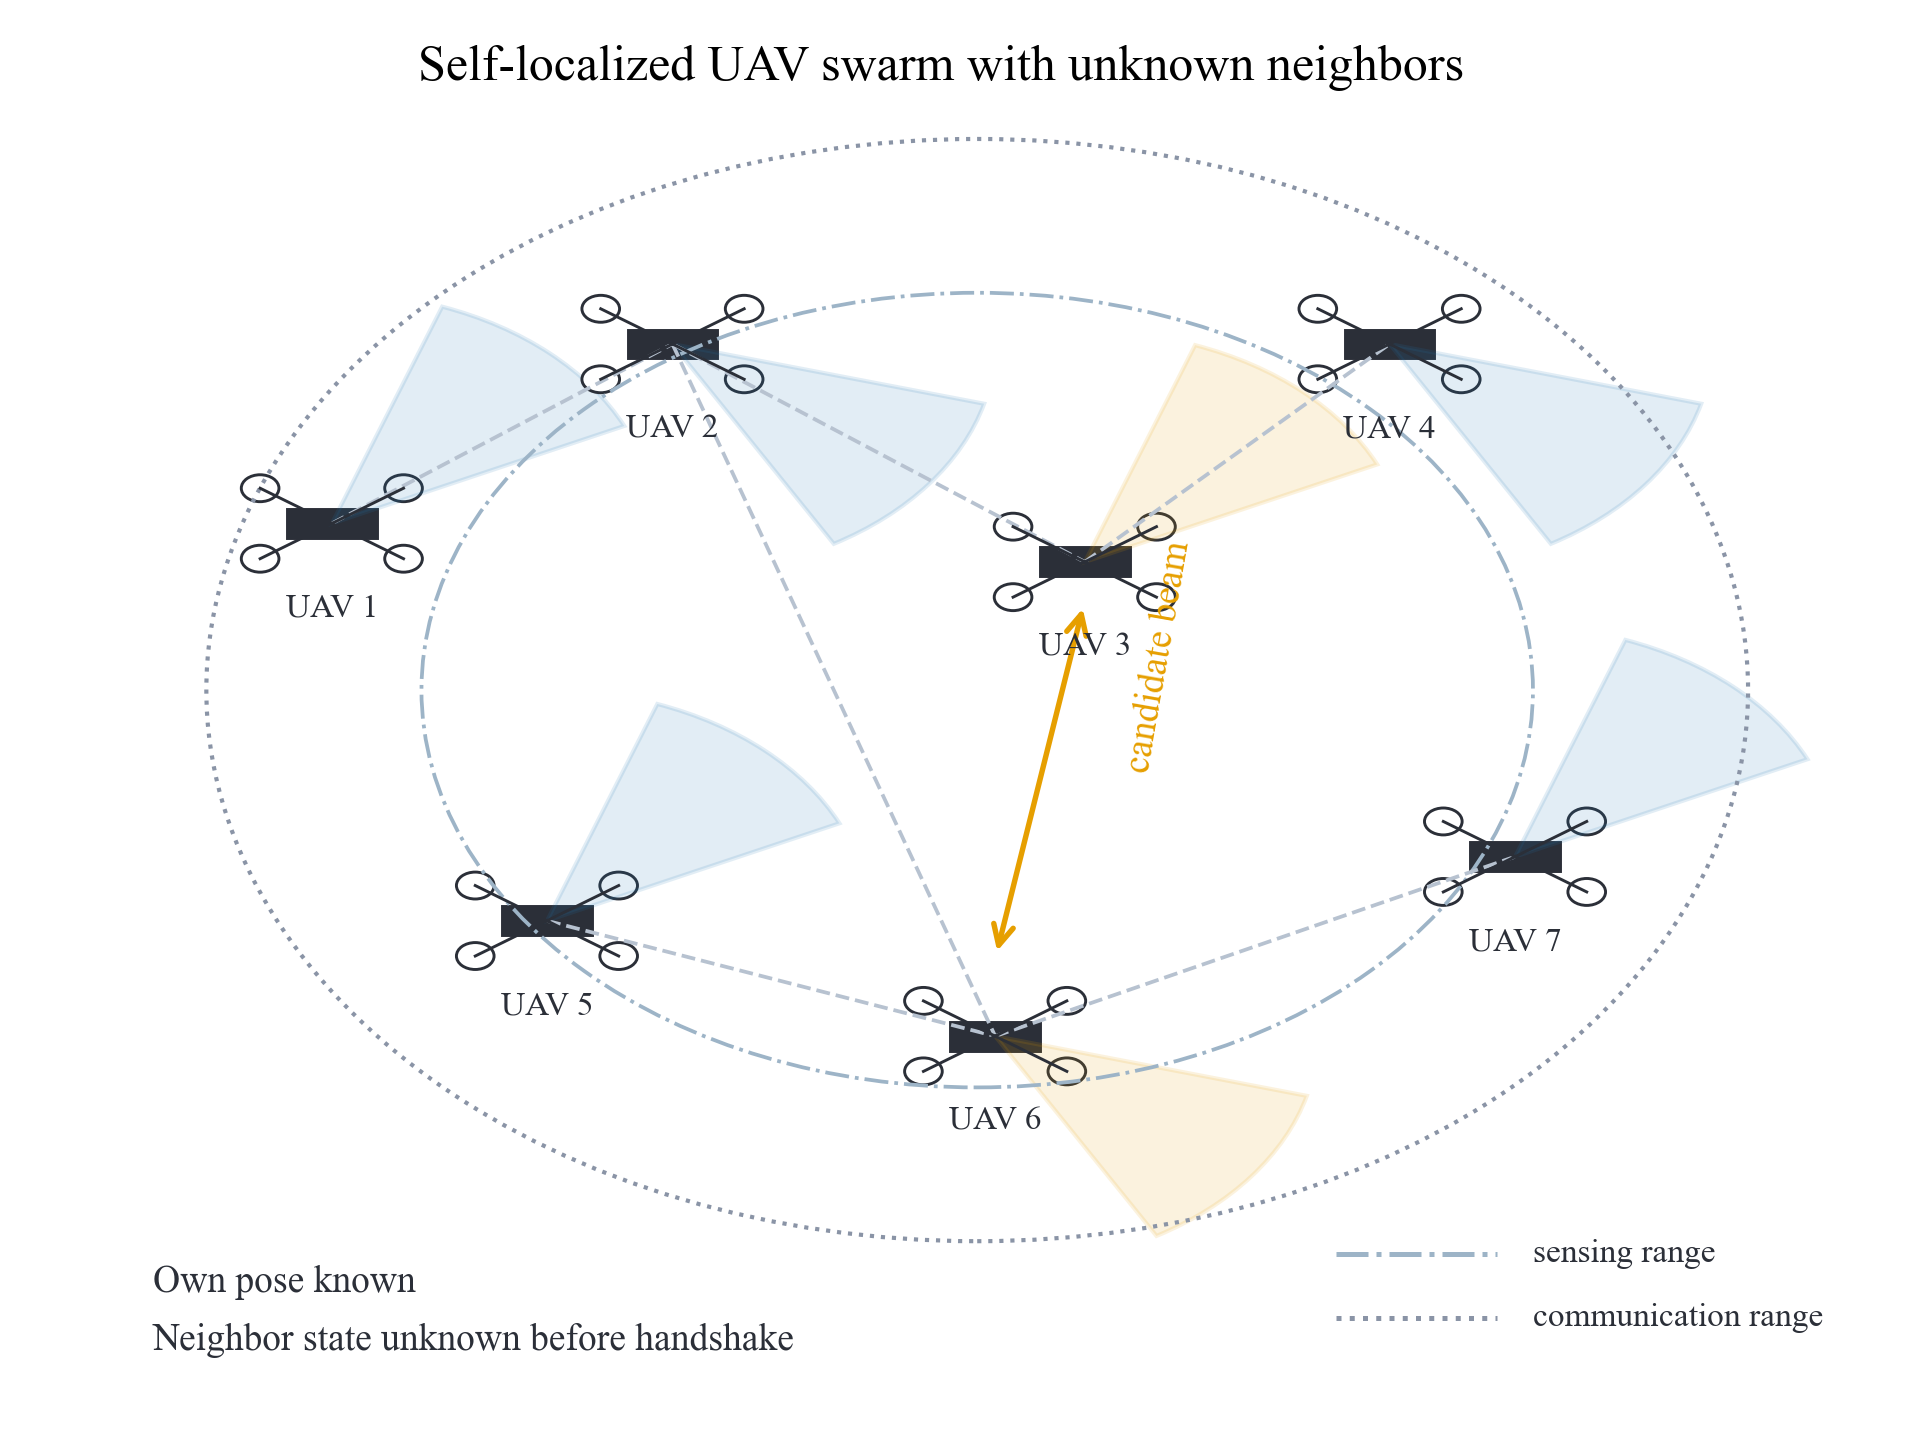
\includegraphics[width=\linewidth]{../../06_analysis/paper_figures/concept/system_model_isac_uav_swarm.png}
  \caption{System model: self-localized UAVs use narrow beams for distributed neighbor discovery while undiscovered neighbor states remain unknown before link-layer handshaking.}
  \label{fig:system_model}
\end{figure}

\section{Related Work}
\subsection{Directional Neighbor Discovery}
Early directional ND work studied probabilistic transmission and listening strategies for nodes with directional antennas \cite{Vasudevan2005DirectionalND}.
Oblivious ND later established a theoretical foundation for distributed directional discovery without prior coordination or synchronization \cite{Chen2017ObliviousND}.
For UAV networks, SkyOrbs introduced a fast three-dimensional directional ND algorithm tailored to aerial scenarios \cite{SkyOrbs2024TMC}.
Our work differs by treating sensing feedback as a link-layer prior and by optimizing finite-time discovery jointly with topology-quality proxies.

\subsection{ISAC-Assisted Beam Management}
ISAC has been used to reduce beam training overhead in vehicular and UAV-assisted systems \cite{Li2024SensingNRV2X,Cui2024SensingUAVBM}.
Recent works also study ISAC-assisted beam rendezvous in airborne networks \cite{Hong2024ISACRendezvous} and predictive beam tracking in multipath channels \cite{Cui2024MultipathISAC}.
Most of these studies focus on physical-layer or beam-management problems between a base station and mobile nodes.
By contrast, this paper targets a fully distributed UAV-UAV ND protocol and uses ISAC only as an imperfect occupancy-prior service exposed to the data-link layer.

\subsection{Learning for Distributed Wireless Protocols}
Multi-agent reinforcement learning and graph neural policies have been studied for wireless resource allocation and distributed channel access \cite{Naderializadeh2021MADRLTWC,Eisen2020REGNN,Guo2022MARLMAC}.
Learning has also appeared in directional ND and beam configuration \cite{Wang2024RLDirectionalND}.
The present draft uses a shared-policy, learning-enhanced distributed policy rather than claiming a complete neural MARL algorithm as the final contribution.
The learning component is used to tune scalable local decision rules that can transfer across swarm sizes.

\section{System Model}
Consider $N$ UAVs moving in a three-dimensional region.
Each UAV $i$ knows its own position $\mathbf{p}_i(t)$, velocity $\mathbf{v}_i(t)$, heading, pitch, and attitude from onboard localization and inertial sensing.
Before neighbor discovery, UAV $i$ does not know the identity, position, velocity, or beam state of an undiscovered UAV $j$.
There is no central controller and no global topology knowledge.

Each UAV has a directional beam codebook $\beamset$ with $B_{\mathrm{az}}$ azimuth cells and $B_{\mathrm{el}}$ elevation cells.
The total number of three-dimensional beam cells is $|\beamset|=B_{\mathrm{az}}B_{\mathrm{el}}$.
A communication edge $(i,j)$ can be discovered in slot $t$ only if (i) the distance is within communication range $\Rc$, (ii) one endpoint transmits and the other receives, and (iii) the selected beams satisfy bidirectional angular alignment within the allowed tolerance.
Discovery is confirmed only by a successful bidirectional narrow-beam handshake.

\subsection{ISAC Prior}
When UAV $i$ probes beam $b$ in a slot, its communication waveform can also provide an ISAC observation of nearby beam cells.
We represent this physical-layer service as a link-layer occupancy observation
\begin{equation}
  z_i^t(b) \in \{0,1\},
\end{equation}
where $z_i^t(b)=1$ indicates that beam cell $b$ is likely occupied by at least one communication-range candidate.
The observation may contain false alarms, missed detections, angular-cell offsets, and staleness.
The sensing range $\Rs$ is evaluated separately from $\Rc$; when $\Rs > \Rc$, sensing beyond the communication range is not assumed to create immediate discoverable neighbors.

Each node maintains a local belief $q_i^t(b)$ for every beam cell.
The belief is updated from ISAC observations using a smoothing factor and decays over time to avoid over-trusting stale evidence.
The belief only biases future beam selection and never bypasses the link-layer handshake.

\section{Protocol Design}
\subsection{\method{}}
\method{} is a distributed slot-level protocol.
In every slot, each UAV chooses among sensing, transmitting, receiving, and idling.
For transmission and reception, the node samples a beam according to a score that combines ISAC occupancy belief, exploration, beam diversity, staleness, and a local topology-value proxy.
The exploration floor prevents permanent exclusion of beam cells that were incorrectly marked empty.

The local topology-value proxy gives larger priority to beams that may establish links for nodes whose discovered degree is below a target degree.
This is not an online computation of global algebraic connectivity.
It is a local rule designed to encourage finite-time formation of a well-connected discovered graph.

\begin{figure}[!t]
  \centering
  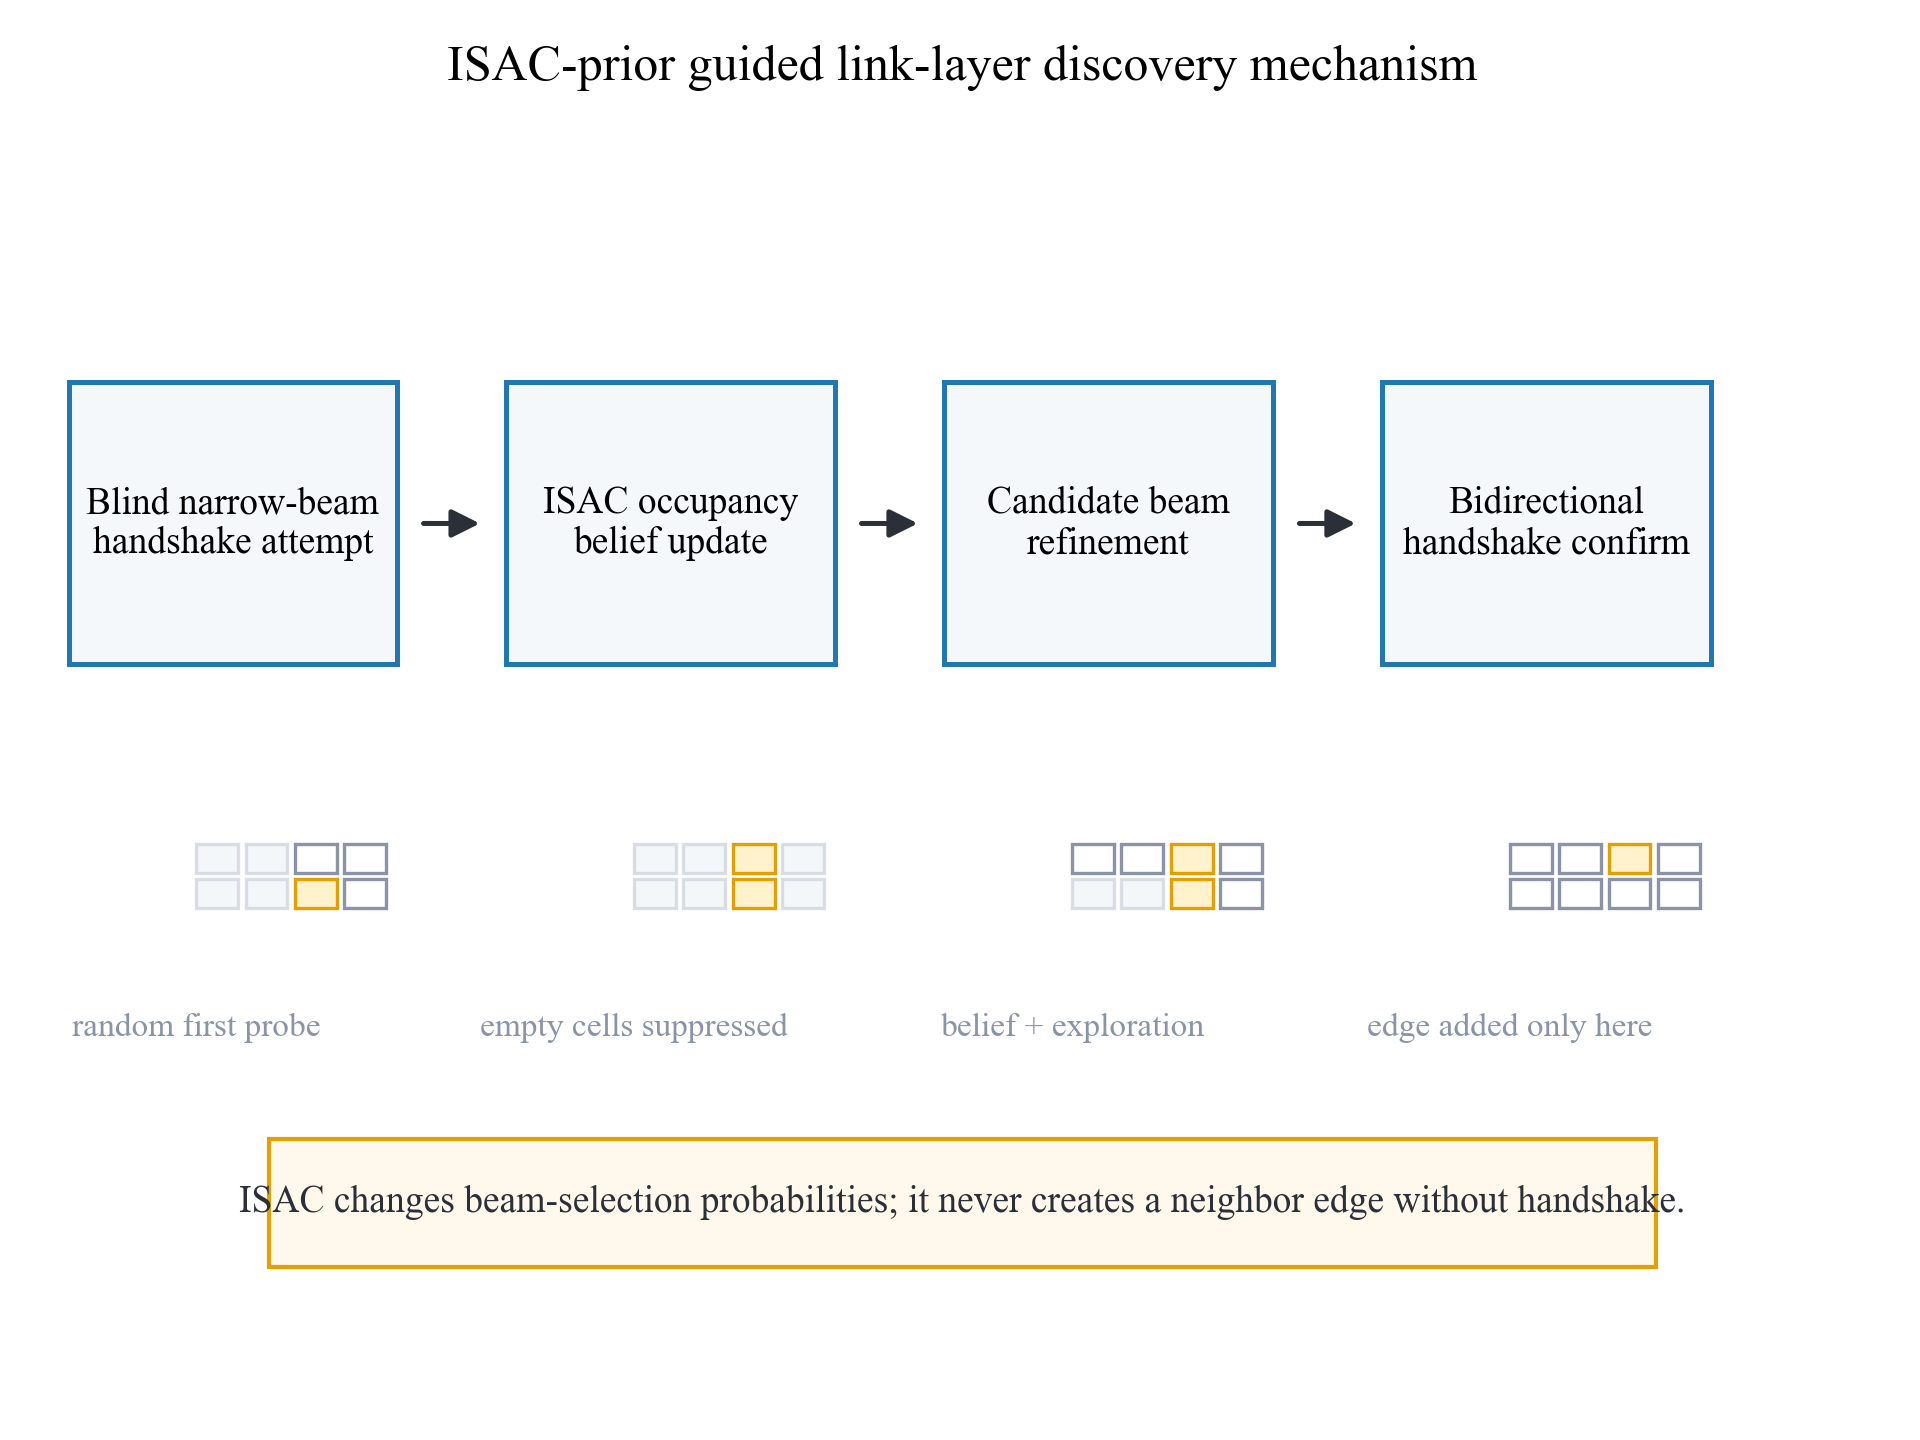
\includegraphics[width=\linewidth]{../../06_analysis/paper_figures/concept/protocol_mechanism_itap_nd.png}
  \caption{Protocol mechanism: an initially blind narrow-beam handshake attempt produces ISAC occupancy feedback, which updates local belief, narrows the candidate beam set, and still requires bidirectional handshake confirmation before adding a neighbor edge.}
  \label{fig:protocol_mechanism}
\end{figure}

\subsection{Learning-Enhanced Shared Policy}
\learnedmethod{} uses the same information boundary as \method{} but tunes the decision weights with a shared policy.
The current implementation uses cross-entropy style shared-parameter search over distributed policy parameters.
This should be described as learning-enhanced policy optimization in the present draft.
Future neural variants can replace the score function with actor-critic, value-decomposition, or graph-neural policies, provided they preserve permutation equivariance and local-observation deployment.

\begin{figure}[!t]
  \centering
  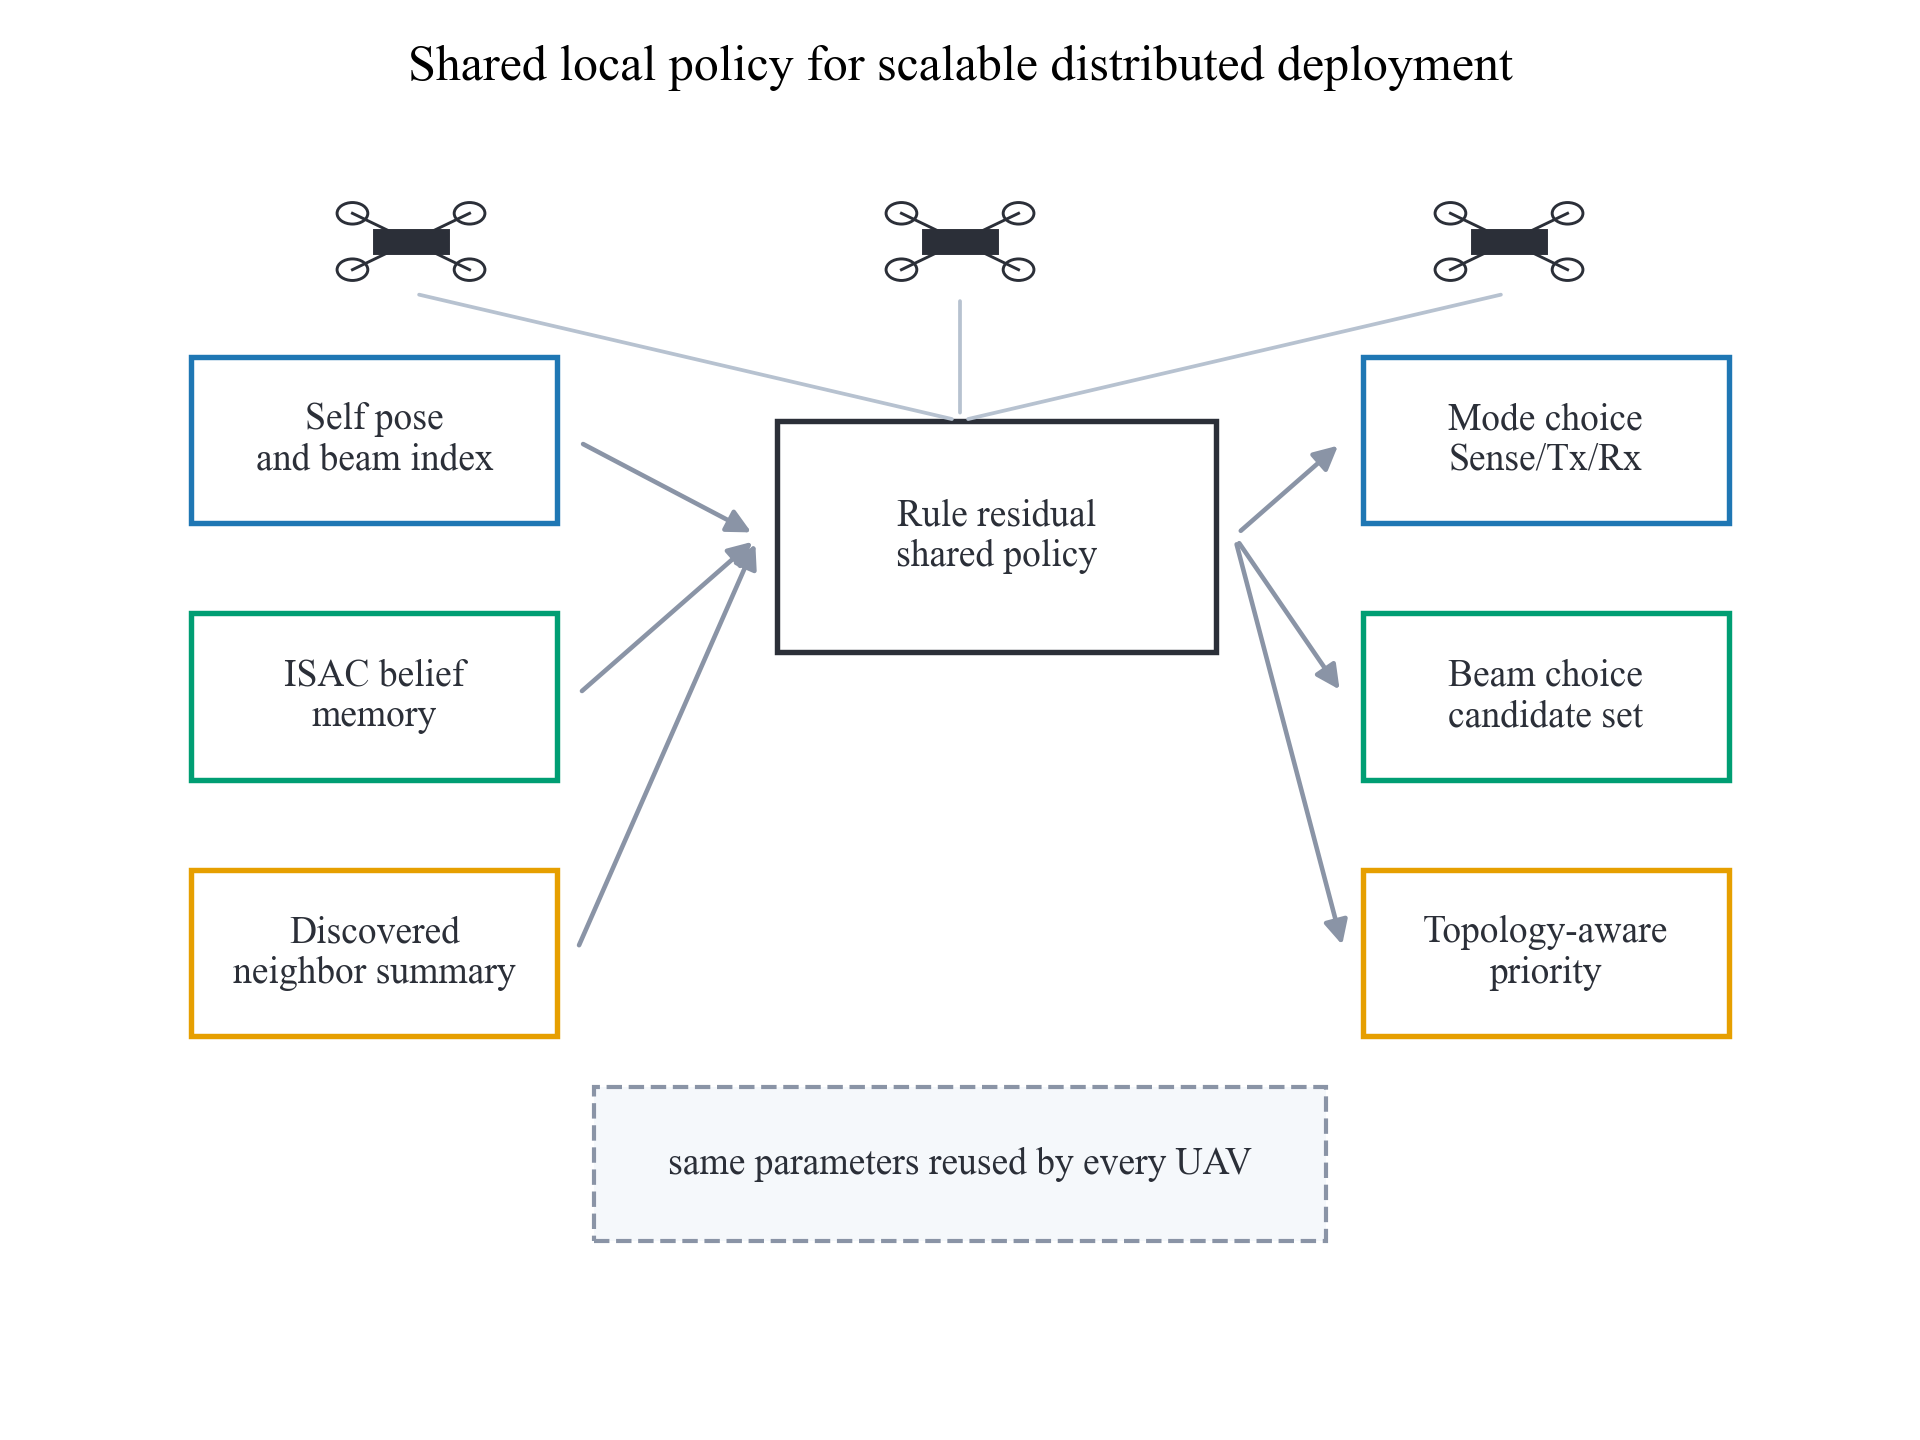
\includegraphics[width=\linewidth]{../../06_analysis/paper_figures/concept/policy_architecture_shared_agent.png}
  \caption{Learning-enhanced shared local policy. The same policy parameters are reused by every UAV, supporting small-scale training and large-scale distributed deployment.}
  \label{fig:policy_architecture}
\end{figure}

\section{Experimental Setup}
\subsection{Mobility and Slot Timing}
The simulation uses dynamic UAV mobility, including Gauss-Markov, random-walk, and random-direction/waypoint variants.
The slot duration is set to 5 ms so that ISAC observations remain meaningful within the mobility timescale.
The primary training configuration uses $N=10$ UAVs and 10-degree beams, and evaluates zero-shot transfer to larger swarms.

\subsection{Baselines}
The comparison set includes uniform random scanning, a SkyOrbs-like directional baseline, learning without ISAC, improved learning without ISAC, and the proposed improved learning with ISAC.
Mechanism ablations remove candidate-set refinement, beam-lock refinement, or topology-aware scoring from the proposed protocol.

\subsection{Metrics}
We report finite-time discovery rate, discovered edge count, mean discovery delay, empty-scan ratio, collision count, largest connected component ratio, and algebraic connectivity $\lambda_2$ of the discovered graph.
Because high-percentile discovery delays can be censored by a finite simulation horizon, the main claims emphasize discovery rate, empty-scan ratio, edge count, and connectivity metrics.

\section{Results and Discussion}
\subsection{Training Convergence}
Fig.~\ref{fig:training_reward} will show the reward/score convergence curve.
Additional training plots report discovery rate, empty-scan ratio, collision count, and connectivity during policy search.

\begin{figure}[!t]
  \centering
  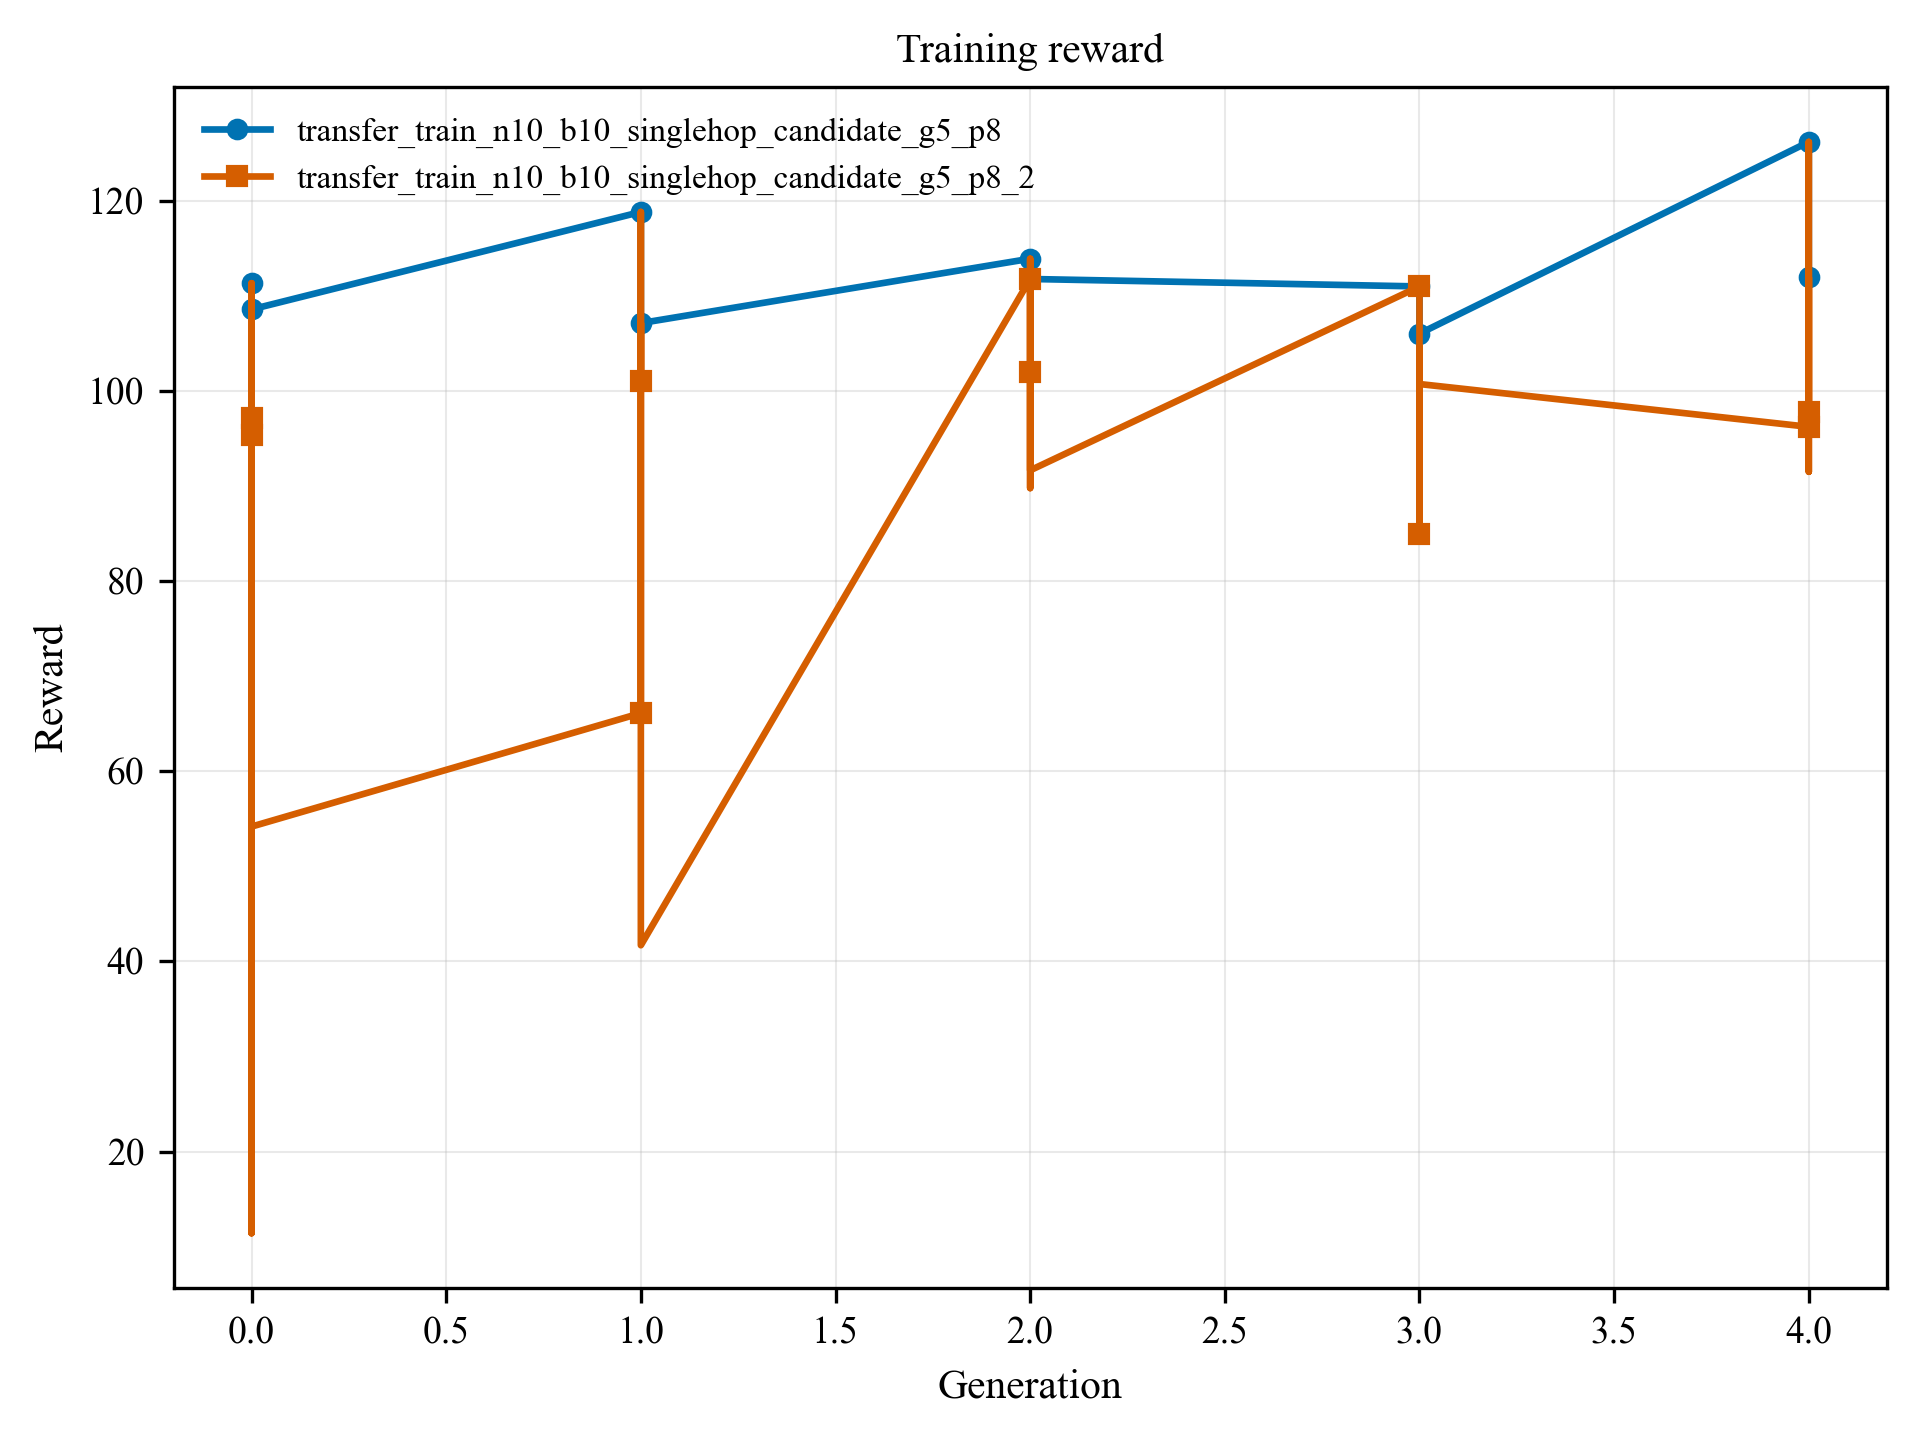
\includegraphics[width=\linewidth]{../../06_analysis/paper_figures/training_round2_candidate/train_reward_curve.png}
  \caption{Training reward convergence for the small-scale shared-policy optimization.}
  \label{fig:training_reward}
\end{figure}

\subsection{Main Transfer Results}
Current round2 results show that the ISAC-assisted improved policy can transfer from $N=10$ and 10-degree beams to larger swarms without fine-tuning.
For example, in the single-hop density-scaled setting at $N=100$ and 10-degree beams, the discovered graph remains connected within the finite horizon, although the finite-time discovery rate is far from complete.
This supports the claim that ISAC priors help form a useful connected topology, but it does not imply that extremely narrow beams are solved.
The round3 multi-seed transfer check confirms this trend at $N=100$.
Under density-preserving scaling, the proposed policy reaches discovery rates of 0.3655, 0.5440, and 0.4568 for 10-, 15-, and 30-degree beams, respectively, while the 5-degree case remains much weaker at 0.0814.
Fixed-area scaling gives a similar trend, indicating that the conclusion is not an artifact of one area-scaling convention.

\begin{figure}[!t]
  \centering
  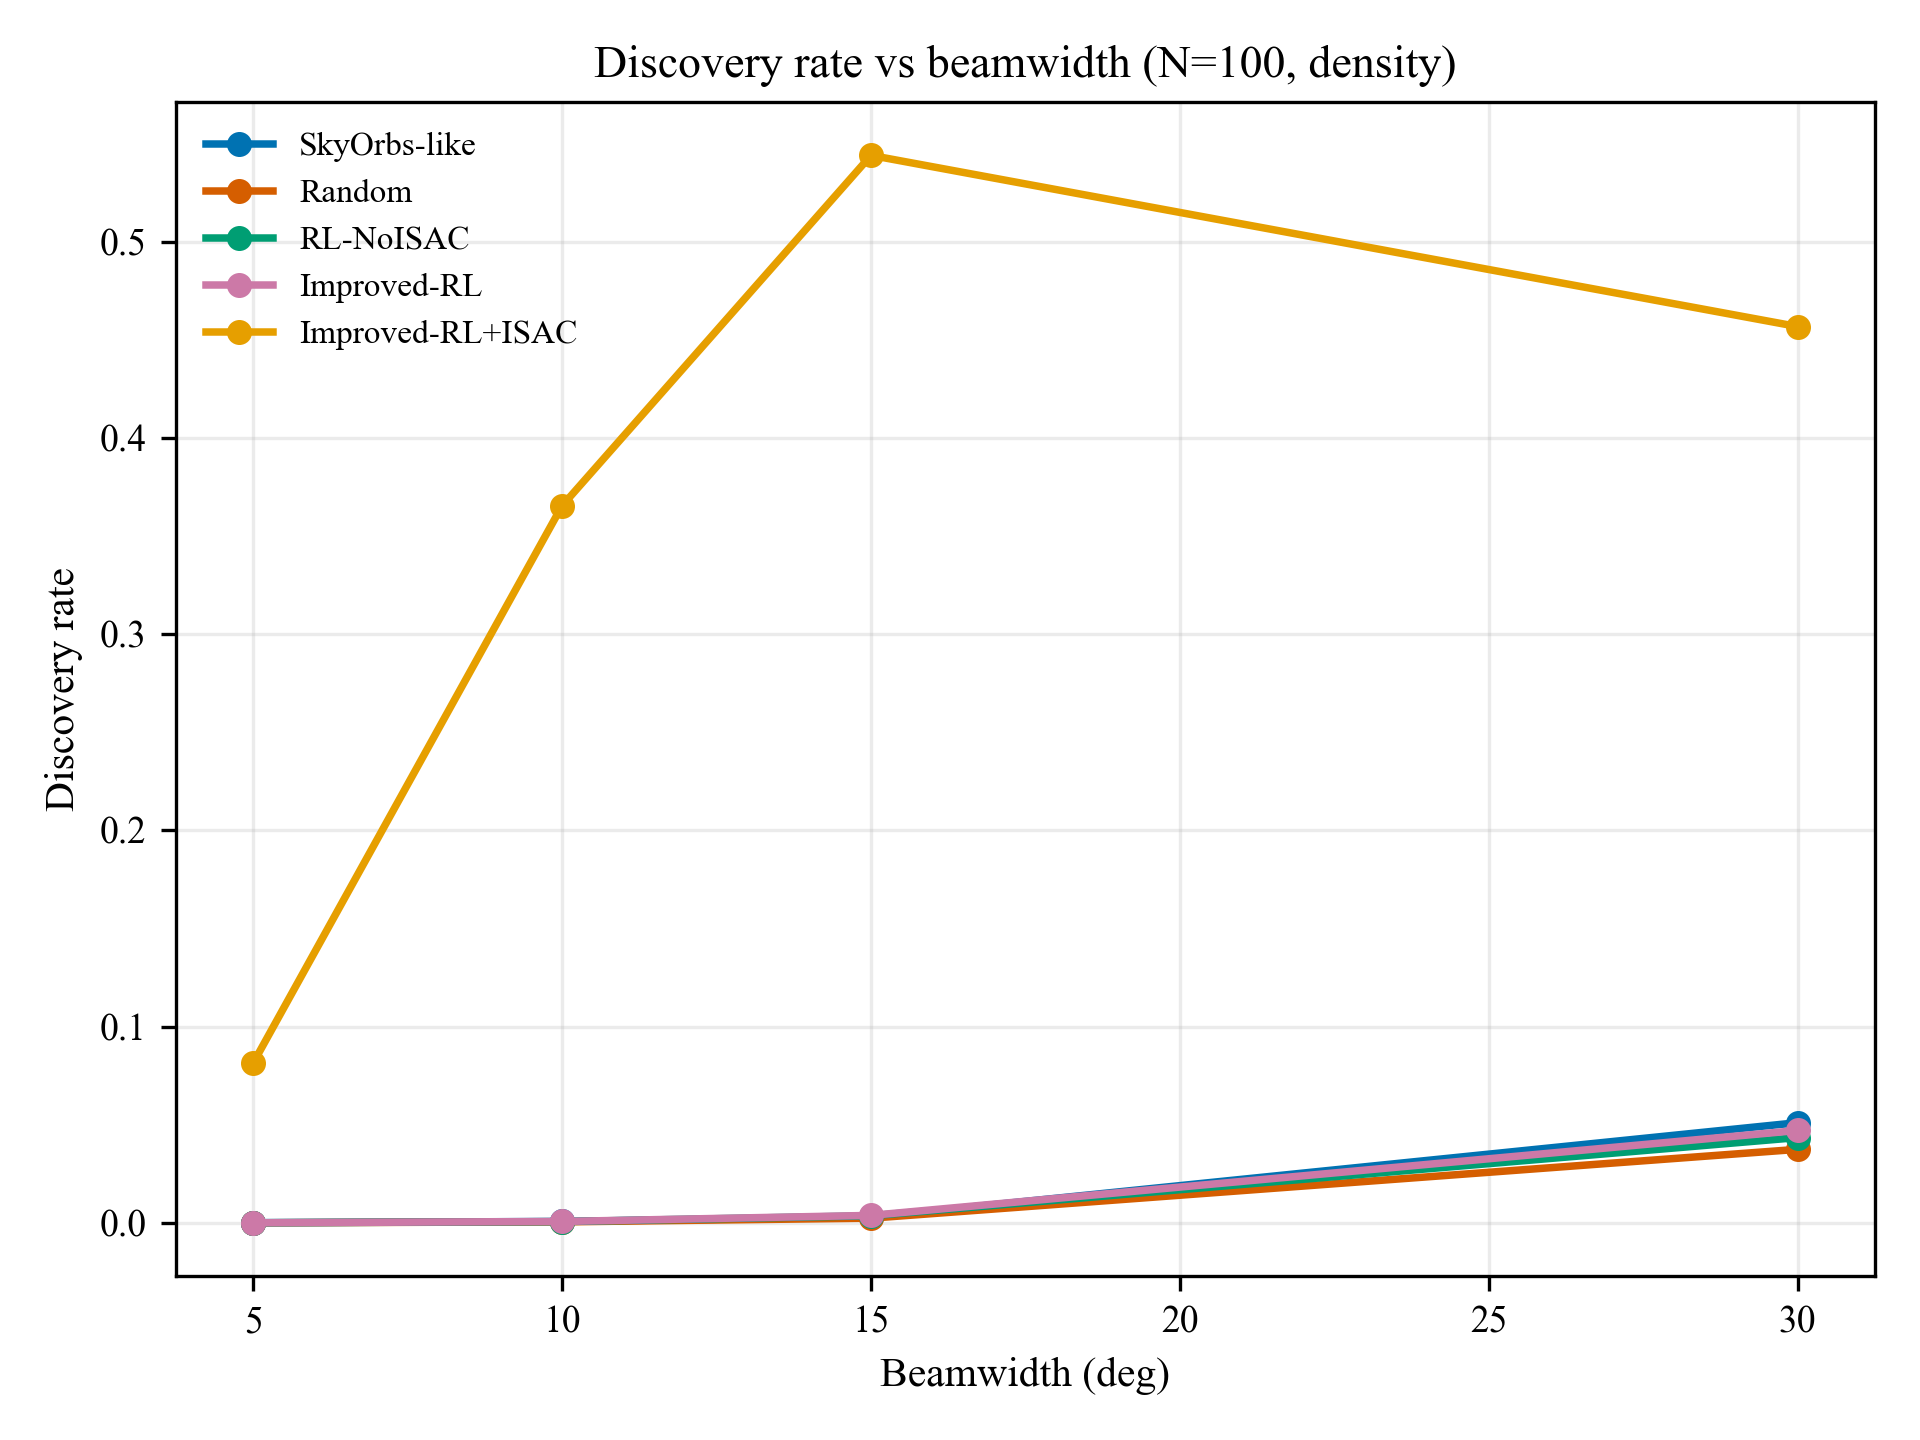
\includegraphics[width=\linewidth]{../../06_analysis/paper_figures/round3_n100_transfer/density_beamwidth_discovery_rate_n100.png}
  \caption{N=100 multi-seed transfer under density-preserving scaling. The policy is trained at N=10 and 10-degree beams, then evaluated without fine-tuning at larger scale and different beamwidths.}
  \label{fig:n100_transfer_density}
\end{figure}

\begin{figure}[!t]
  \centering
  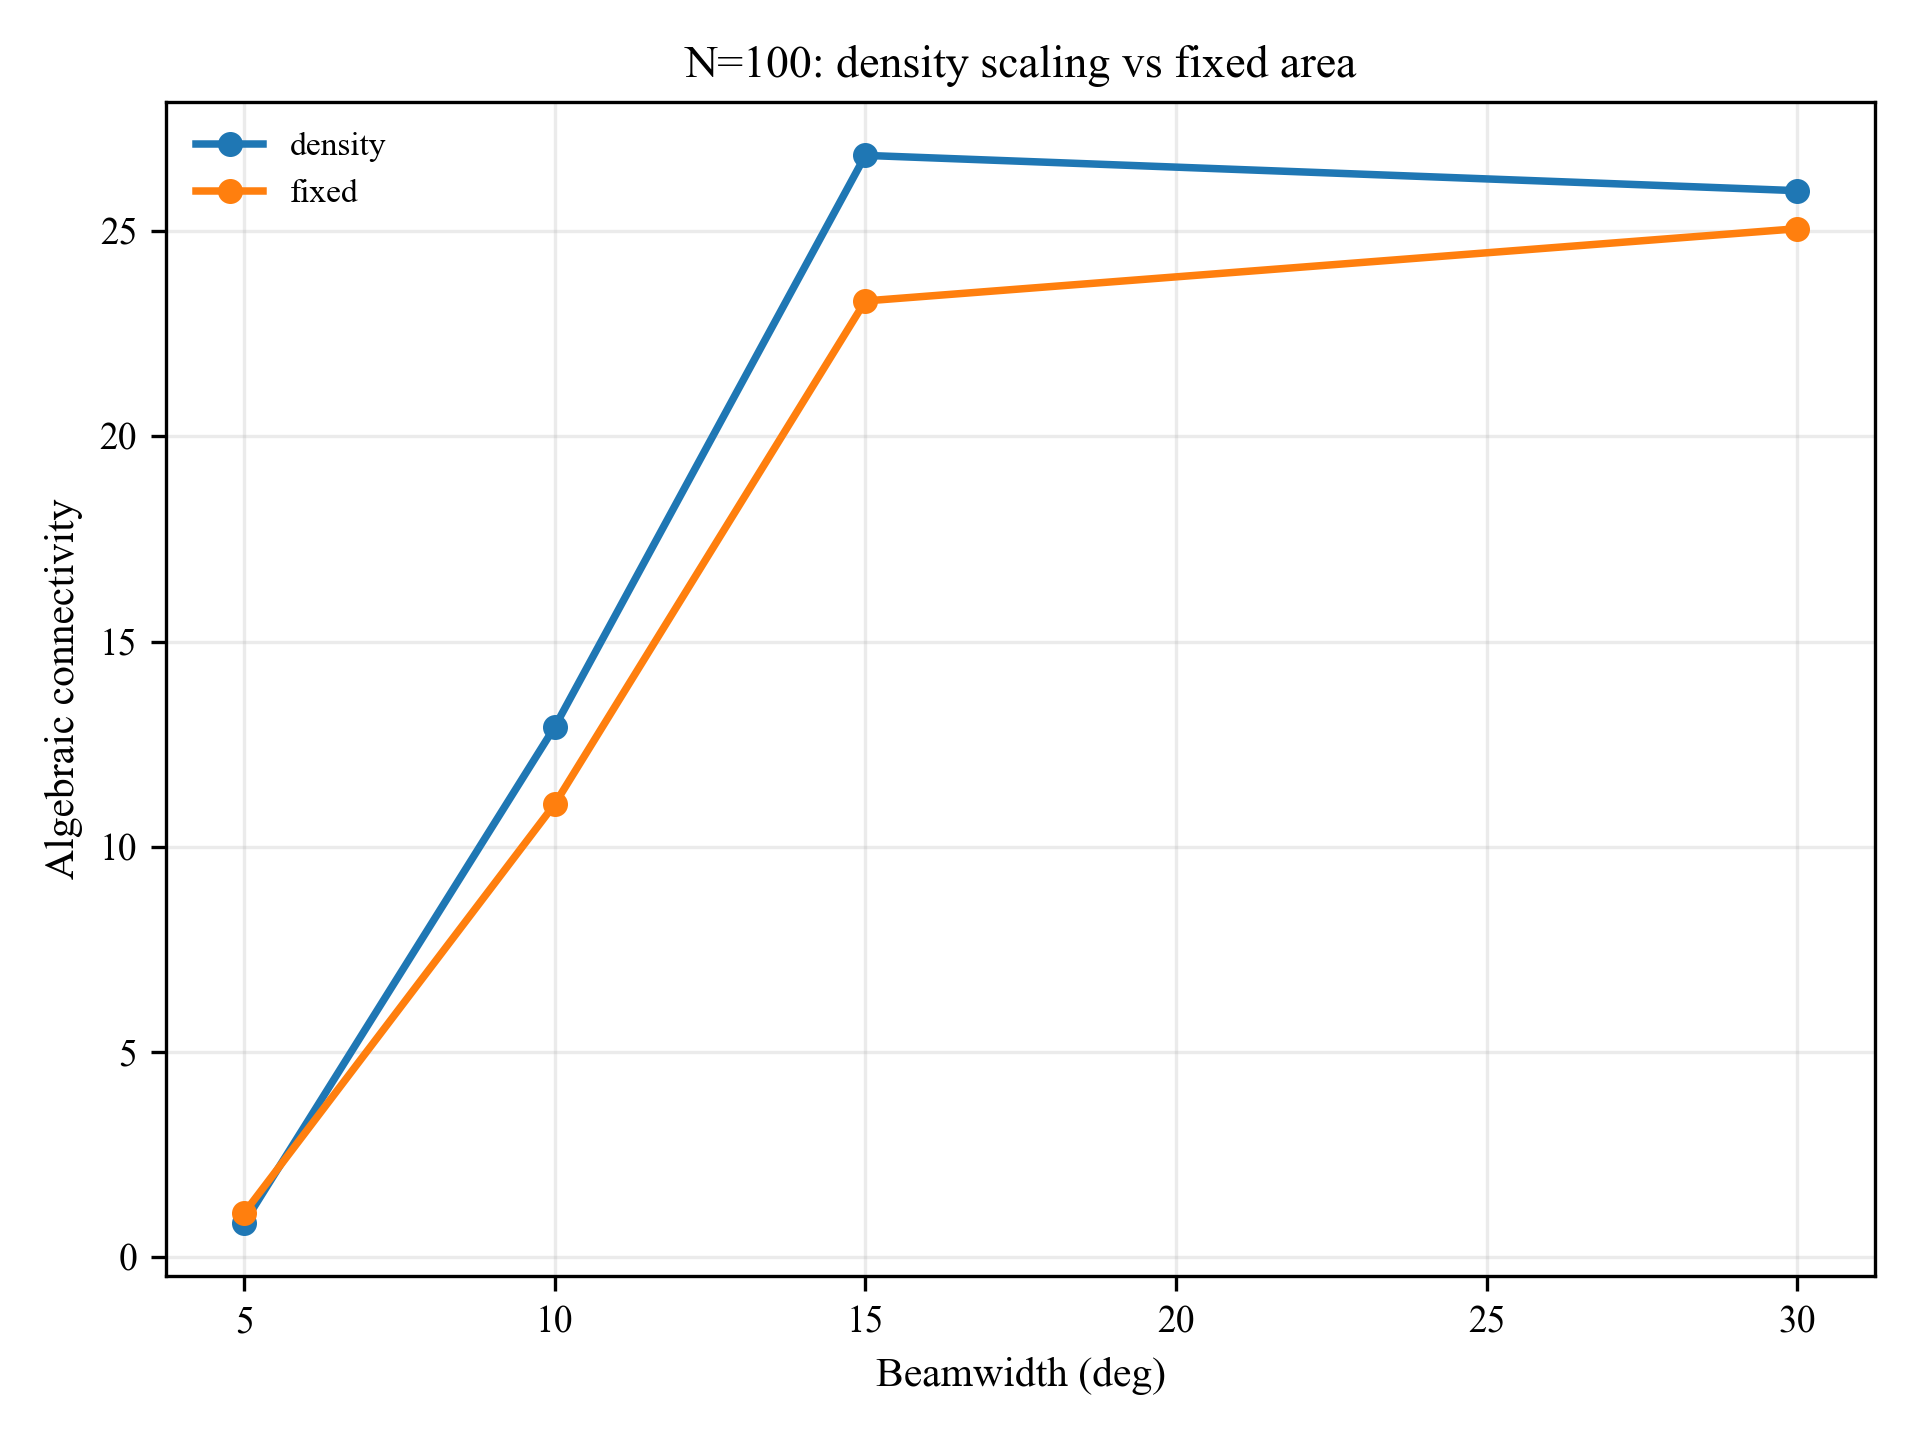
\includegraphics[width=\linewidth]{../../06_analysis/paper_figures/round3_n100_transfer/area_scale_n100_lambda2.png}
  \caption{Density-preserving versus fixed-area scaling at N=100. Both settings show similar connectivity trends, with 10-30 degree beams being the most useful operating region in the current finite horizon.}
  \label{fig:n100_area_scale}
\end{figure}

\subsection{Range, Error, and Mechanism Robustness}
Round3 experiments are running to complete three reviewer-critical checks:
\begin{itemize}
  \item $\Rc/D$ and $\Rs/\Rc$ sensitivity, where $D$ is the region diagonal.
  \item ISAC false-alarm, missed-detection, and angular-cell-offset robustness.
  \item Mechanism ablations for candidate-set refinement, beam-lock refinement, and topology-aware scoring.
\end{itemize}
The manuscript should only make strong robustness claims after these results are aggregated and plotted.
The range sweep shows that sensing range is most useful when it approaches the communication range.
At $\Rc/D=0.65$, increasing $\Rs/\Rc$ from 0.5 to 0.75 improves the proposed policy's discovery rate from 0.2628 to 0.3569.
Increasing $\Rs$ beyond $\Rc$ does not provide additional gain for communication-range neighbor discovery, which is consistent with the model assumption that only communication-range neighbors can be immediately confirmed by handshake.

\begin{figure}[!t]
  \centering
  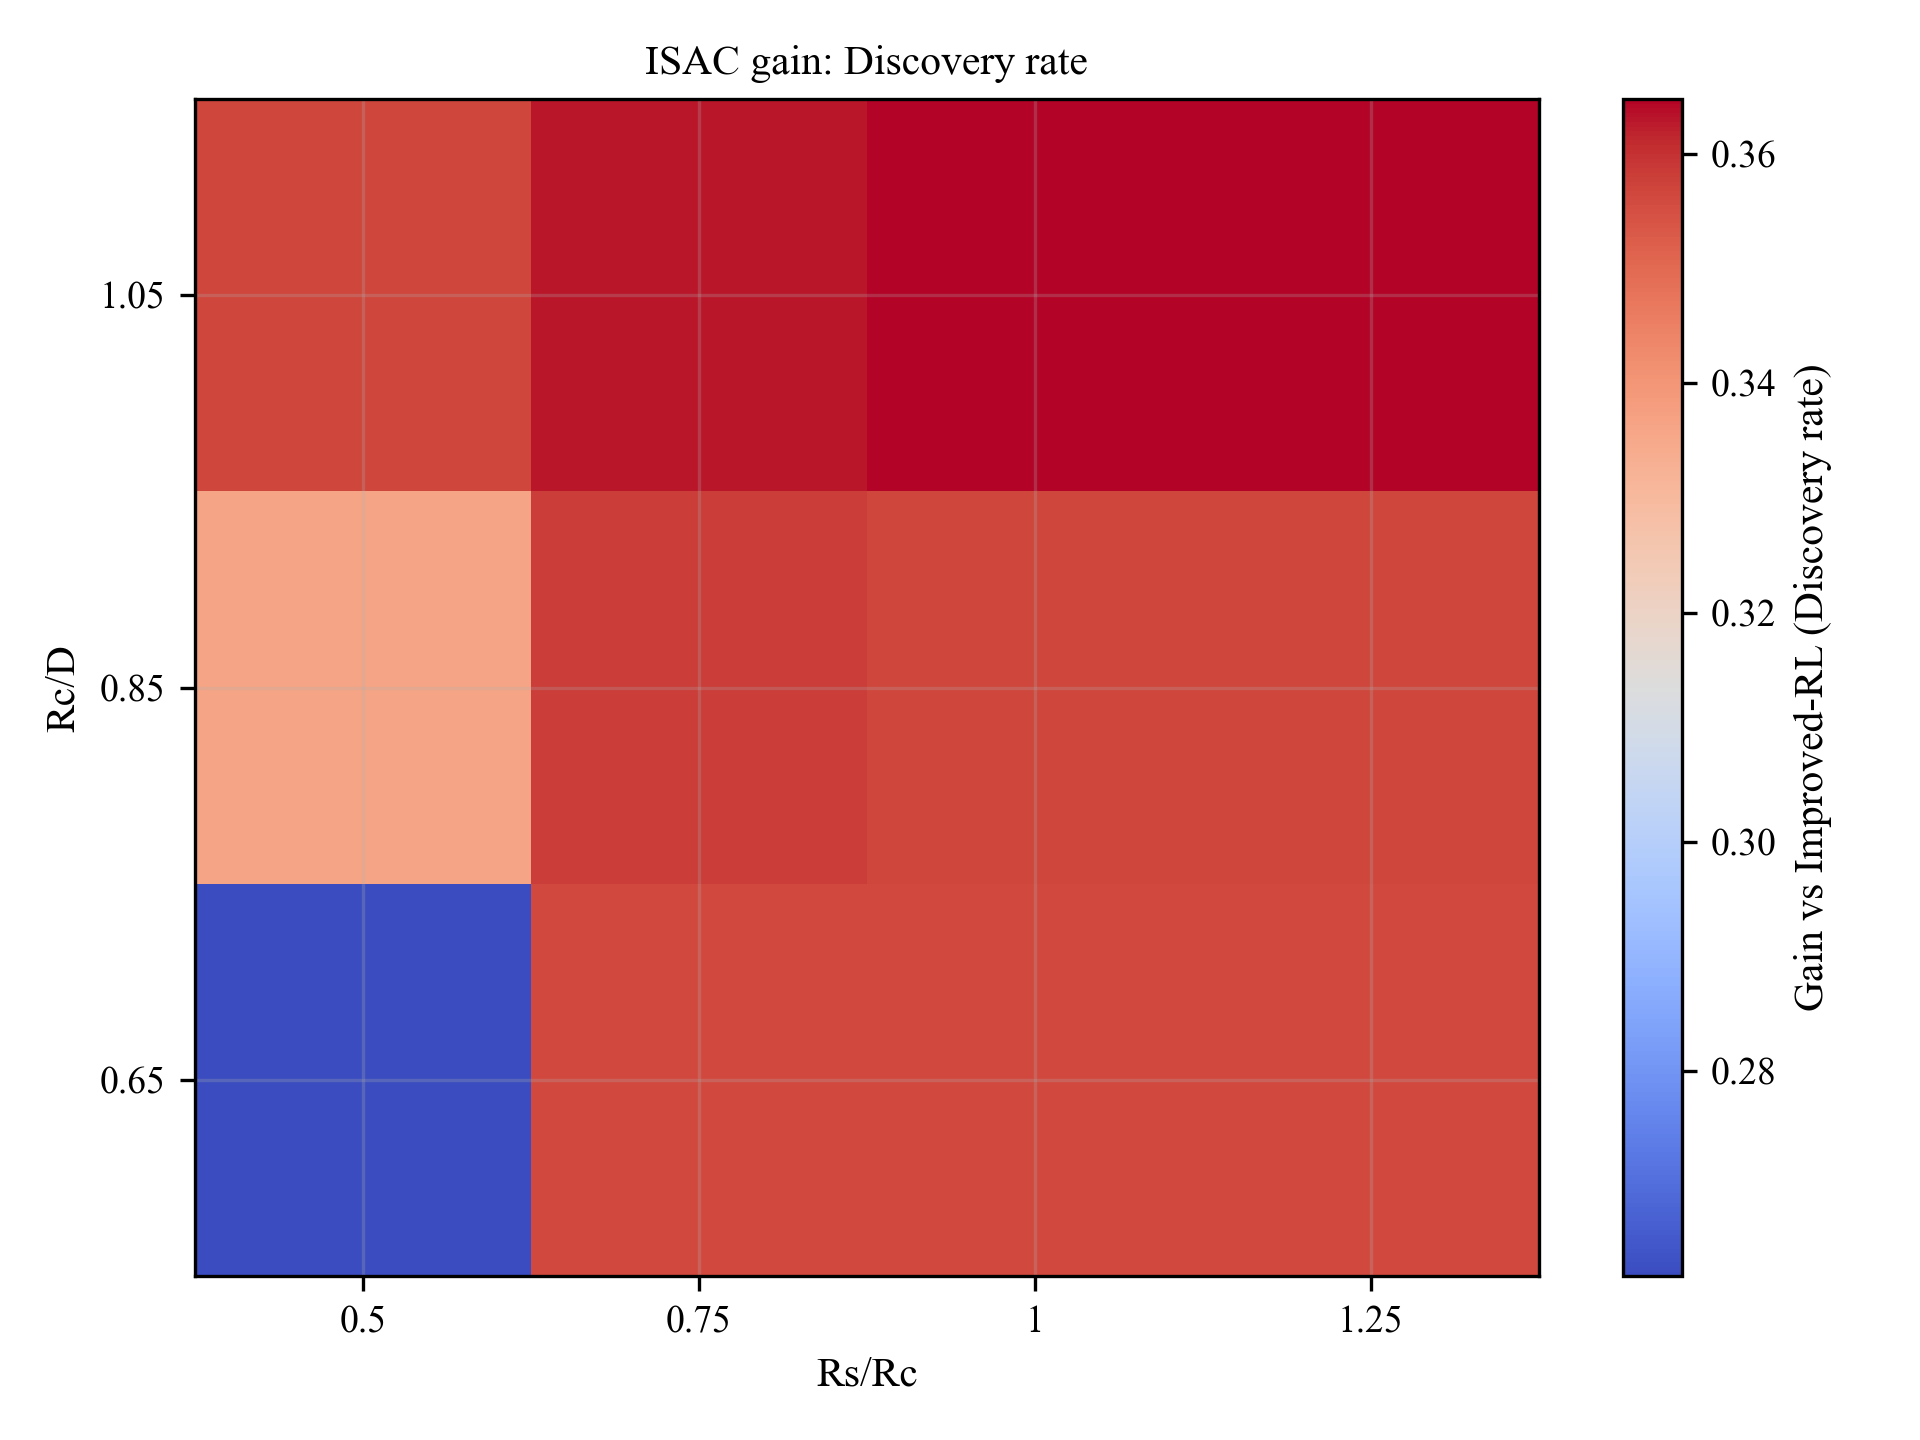
\includegraphics[width=\linewidth]{../../06_analysis/paper_figures/round3_robustness/range_gain_discovery_n100_b10.png}
  \caption{Range sensitivity at N=100 and 10-degree beams. The heatmap reports discovery-rate gain of the ISAC-assisted policy over the improved no-ISAC baseline across communication-range and sensing-range ratios.}
  \label{fig:range_gain_heatmap}
\end{figure}

The mechanism ablation completed first.
At $N=100$ and 10-degree beams, removing the ISAC-driven candidate-set refinement reduces the discovery rate from 0.3655 to 0.0313 and drives the discovered graph connectivity to nearly zero.
Removing topology-aware scoring or beam-lock refinement causes a smaller degradation, suggesting that candidate-set formation is the dominant mechanism in the current protocol.

\begin{figure}[!t]
  \centering
  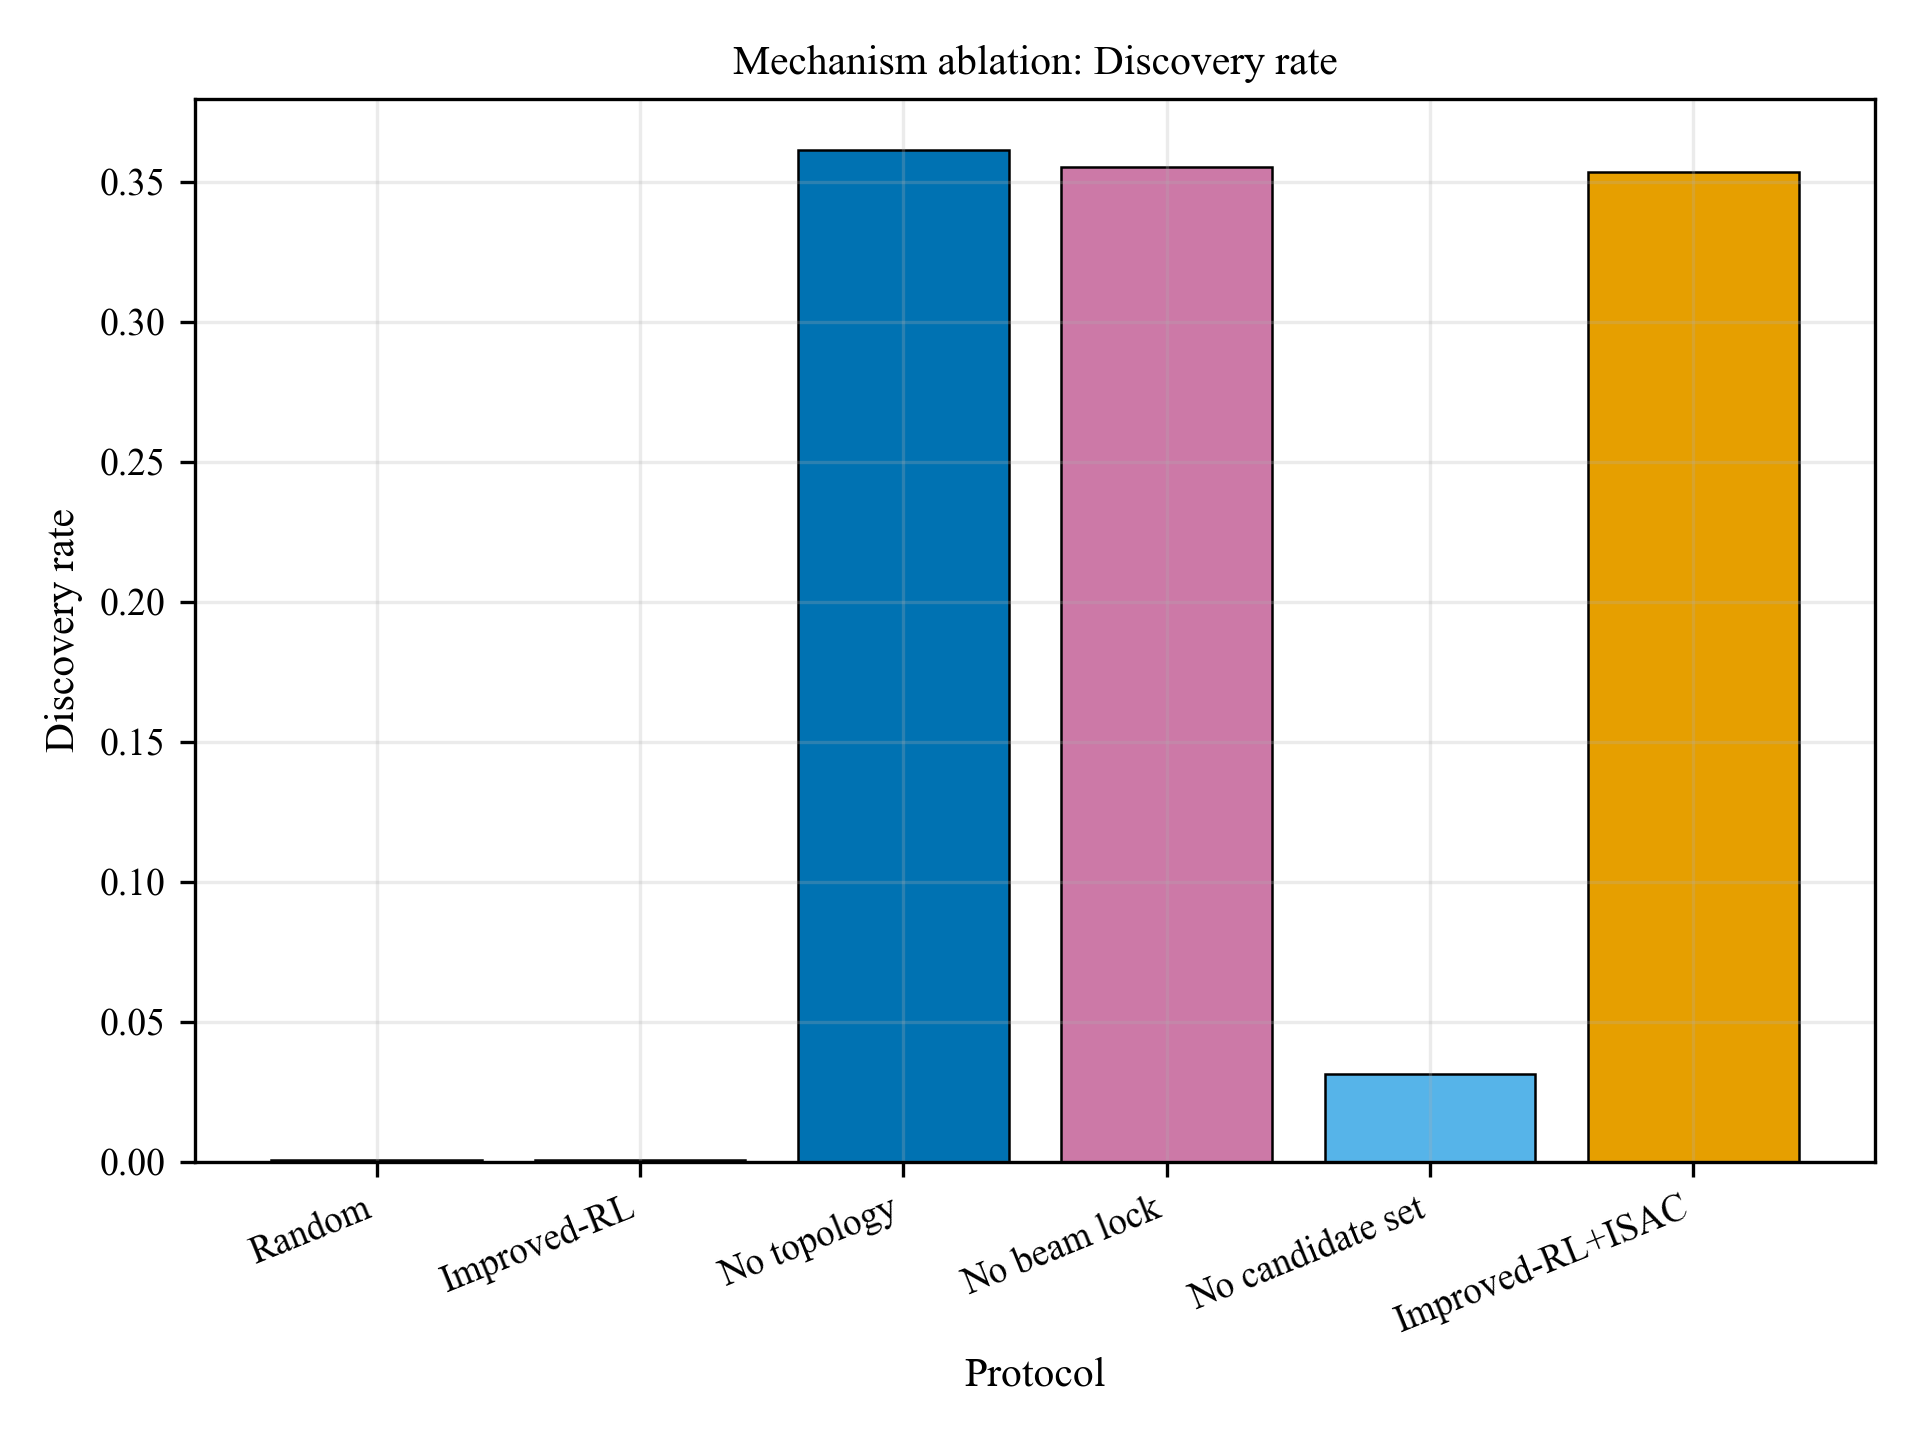
\includegraphics[width=\linewidth]{../../06_analysis/paper_figures/round3_robustness/ablation_discovery_n100_b10.png}
  \caption{Mechanism ablation at N=100 and 10-degree beams. Candidate-set refinement is the dominant contributor to finite-time discovery in the current implementation.}
  \label{fig:ablation_discovery}
\end{figure}

\section{Limitations}
This draft has four important limitations.
First, the current learning component is a shared-policy parameter optimization workflow, not yet a full MAPPO, QMIX, or graph neural MARL implementation.
Second, the SkyOrbs comparison is a SkyOrbs-like baseline rather than a strict reproduction of the complete original algorithm.
Third, ISAC is represented by an abstract beam-cell occupancy prior; physical waveform design and estimator implementation are outside the scope.
Fourth, extremely narrow beams at 3 and 5 degrees remain a stress region and should be discussed as such.

\section{Conclusion}
This paper studies ISAC-assisted narrow-beam neighbor discovery for fully distributed UAV swarms.
The central idea is to use ISAC not as an oracle, but as an imperfect beam-cell prior that reduces empty scanning while preserving link-layer handshake confirmation.
The current simulation workflow supports the feasibility of this direction and identifies the robustness experiments needed for a submission-quality TWC/TCOM manuscript.

\section*{Acknowledgment}
TODO: Add funding and contributor information.

\bibliographystyle{IEEEtran}
\bibliography{references}

\end{document}
